\documentclass[preprint, 12pt]{elsarticle}

%% Use the option review to obtain double line spacing
%% \documentclass[preprint,review,12pt]{elsarticle}

%% Use the options 1p,twocolumn; 3p; 3p,twocolumn; 5p; or 5p,twocolumn
%% for a journal layout:
%% \documentclass[final,1p,times]{elsarticle}
%% \documentclass[final,1p,times,twocolumn]{elsarticle}
%% \documentclass[final,3p,times]{elsarticle}
%% \documentclass[final,3p,times,twocolumn]{elsarticle}
%% \documentclass[final,5p,times]{elsarticle}
%% \documentclass[final,5p,times,twocolumn]{elsarticle}

%% The graphicx package provides the includegraphics command.
\usepackage{graphicx}
\usepackage{subcaption}
%% The amssymb package provides various useful mathematical symbols
\usepackage{amssymb}
\usepackage{siunitx}
%%\usepackage{authblk}
%% The amsthm package provides extended theorem environments
%% \usepackage{amsthm}

%% The lineno packages adds line numbers. Start line numbering with
%% \begin{linenumbers}, end it with \end{linenumbers}. Or switch it on
%% for the whole article with \linenumbers after \end{frontmatter}.
\usepackage{lineno}
\usepackage[]{hyperref}

%% natbib.sty is loaded by default. However, natbib options can be
%% provided with \biboptions{...} command. Following options are
%% valid:

%%   round  -  round parentheses are used (default)
%%   square -  square brackets are used   [option]
%%   curly  -  curly braces are used      {option}
%%   angle  -  angle brackets are used    <option>
%%   semicolon  -  multiple citations separated by semi-colon
%%   colon  - same as semicolon, an earlier confusion
%%   comma  -  separated by comma
%%   numbers-  selects numerical citations
%%   super  -  numerical citations as superscripts
%%   sort   -  sorts multiple citations according to order in ref. list
%%   sort&compress   -  like sort, but also compresses numerical citations
%%   compress - compresses without sorting
%%
%% \biboptions{comma,round}

% \biboptions{}

\DeclareSIUnit{\Wsqcm}{\watt\per\square\centi\meter}
\journal{Journal Name}

\begin{document}

\begin{frontmatter}

%% Title, authors and addresses

%\title{Particle--in--cell simulation of the dynamics of short--pulse laser
%irradiated multilayer targets and x--ray reflectometry diagnostics.}

\title{Theoretical study on grazing-incidence x-ray scattering of  surfaces upon high-intensity laser irradiation}


%% use the tnoteref command within \title for footnotes;
%% use the tnotetext command for the associated footnote;
%% use the fnref command within \author or \address for footnotes;
%% use the fntext command for the associated footnote;
%% use the corref command within \author for corresponding author footnotes;
%% use the cortext command for the associated footnote;
%% use the ead command for the email address,
%% and the form \ead[url] for the home page:
%%
%% \title{Title\tnoteref{label1}}
%% \tnotetext[label1]{}
%% \author{Name\corref{cor1}\fnref{label2}}
%% \ead{email address}
%% \ead[url]{home page}
%% \fntext[label2]{}
%% \cortext[cor1]{}
%% \address{Address\fnref{label3}}
%% \fntext[label3]{}


%% use optional labels to link authors explicitly to addresses:
%% \author[label1,label2]{<author name>}
%% \address[label1]{<address>}
%% \address[label2]{<address>}

\author[1]{M. Banjafar}
\author[2]{L. Randolph}
\author[3]{T. Kluge}
\author[3]{M. Bussmann}
\author[1]{A .P. Mancuso}
\author[3]{T. E. Cowan}
\author[1]{C. Fortmann-Grote}
\author[2]{C. Gutt}
\author[1]{M. Nakatsutsumi}

%%\affil[1]{European XFEL GmbH, }

\address[1]{European XFEL GmbH, Holzkopple 4, 22869 Schenefeld, Germany}
\address[2]{Department of Physics, University of Siegen, D-57072 Siegen, Germany}
\address[3]{Helmholtz-Zentrum Dresden-Rossendorf, Bautzner Landstraße 400, 01328 Dresden, Germany}

\begin{abstract}
%% Text of abstract
  Interaction of solid materials with laser pulses
  produces warm dense matter under controlled laboratory conditions.
  Multilayer targets of alternating high and low Z material layers of a few
  nanometer thickness open the possibility
  to study the laser--matter interaction dynamics as a volumetric effect by
  observing the multilayer Bragg peak in a x--ray reflectometry experiment.
  Here, we present particle--in--cell simulations of
  the laser and multilayer target interaction and subsequent calculations of
  the reflectivity as a
  function of reflection angle and various time delays between the optical pump
  and the x--ray probe pulse delivered by an x--ray free--electron laser.
  Using the same methodology, we also calculate the diffuse x--ray scattering
  signal.
  We demonstrate that the combined measurement of reflectivity and
  diffuse scattering provides valuable information about the evolution of
  electron density gradients, temperature and ionization as a function of target
  depth and pump--probe time delay and Bragg peak position.
\end{abstract}

\begin{keyword}
Short pulse laser--matter interaction \sep particle--in--cell simulations \sep x--ray
diagnostics \sep x--ray free--electron laser
%% MSC codes here, in the form: \MSC code \sep code
%% or \MSC[2008] code \sep code (2000 is the default)
\end{keyword}
\end{frontmatter}

%%
%% Start line numbering here if you want
%%
\linenumbers
\begin{verbatim}
Carsten:
* Abstract to be iterated when rest of the text comes into shape.}
* What figures will go in the paper?
Thomas:
  * Experimental description should focus on giving the physical
  motivation of why we want to do surface diffraction at all
  * Simulation part should focus on showing
    (1) the qualitative plasma physics we expect
    (2) the differences between codes with respect to
      (a) different physics included (e.g. comparing with and without
      ionization, with and withou collisions etc)
      (b) different models, e.g.
        i) TF vs. Direct impact ionization
        ii) large collision frequency vs. low collision frequency
        iii) comparing a constant Coulomb logarithm vs. a T-dependent one
        iV) hydro vs. PIC
      (c) different model implementations (e.g. TF and ADK are different
      in PICLS and PIConGPU)
    (3) lay the foundation in showing what plasma physics is important and
    what the uncertainties in the numerical modeling are, so that in the
    scattering part one can focus on showing how to measure the physics
    and validate the codes
  * The scattering part has to derive much more stringent the connection
  between the measured quantities (e.g. beta, change of max(Q) position,
  fourier transform/rings) and plasma physical quantities (e.g. what
  exactly are slow/fast dynamics and how do they imprint on the speckle
  contrast? surface ripple correlation changes - where do they come from
  (should be explained in the sim-part) and how do the show up in the
  signal, what exactly expands and how/why does it imprint on the signal,
  what is the plasma physics measured by the ring-analysis?...)
\end{verbatim}
\begin{verbatim}
TODOS:
  * Abstract
  info, structure the paper, suggestions below
  * Introduction:
    -Motivation
    - Intensity regime -> WDM, some words about prepulse in high-power laser
    experiments
  * Schematic experiment setup (use figure from talk)
  * Methods:
    - PIC: which code(s), only short, give references. briefly discuss
  collisional ionization and collisions.
    - reflectometry calculations from PIC results
  * Results:
    - electron density plots, maybe video for supplemental material (only Ta-Al,
    or also Ta-Si?)
    - electron density profiles, difference betwen codes (do we want to show
    here, is it checked?)
    - reflection curves, diffuse scattering (?)
  * Discussion
  * Summary, Outlook
\end{verbatim}

%% main text
\section{Introduction}
\label{S:1}

High--intensity laser--matter interaction with solid density targets opens
broad applications such as high--harmonic generation \cite{}, laboratory
astrophysics \cite{}, materials research \cite{}, laser driven fusion
\cite{}, particle acceleration \cite{}, and optical applications such as plasma
mirrors \cite{}.
Laser--matter coupling is largely dominated by the instantaneous electron density.
Substantial ionization due to \ldots can already be observed at
non--relativistic laser intensities (\SI{\ll
e18}{\Wsqcm}). A femtosecond optical laser pulse at moderate intensities
(\SIrange{e14}{e16}{\Wsqcm}) impinging on a thin
metal foil with a few tens of \si{\nm} thickness produces pressures in excess of
\SI{1}{\mega\bar}. Under such conditions, warm dense matter (WDM) forms
with electron densities close to solid density and temperatures of a few
thousand to a few ten thousand \si{\K}. This is also the mechanism of a plasma
mirror, where a pre--pulse of  \SI{\approx e16}{\Wsqcm} makes the target surface
highly reflective and thereby improves the temporal contrast and focussing of
the main pulse \marginpar{Is this correct?}.
It is thus of strong interest to understand
the physics of WDM and in particular the spatial structure on a \si{\nm} scale
and the electron dynamics in the \si{\fs} regime
because these in turn determine the interaction with the peak
part of the relativistic pulse.
Beyond this technological motivation, there is also fundamental interest in WDM
due to its abundance in many astrophysical objects \cite{Nettelmann2008a}
such as planetary
interiors (including the earth's), and stellar atmospheres. The regime of WDM
is also crossed by the trajectory of inertial confinement fusion targets \cite{Lindl2004}, adding
again to the technologically driven interest in this subject.

WDM is a particularly challenging state of matter both from the experimental and from the
theoretical perspective. Being a highly transient state, extremely high temporal
and spatial resolution is required to probe the target's structure and dynamics
using e.g. pulsed x--ray sources. Recently, laser--plasma driven x--ray sources
and free--electron lasers have become the state--of--the--art sources for this
research \cite{Lee2003, Lee2003a}.
X--ray reflectometry (XRR) and grazing incidence x--ray diffraction (GIXD) \cite{TBC} are particularly
sensitive to the sample electron distribution in the plane and in the direction
perpendicular to the target surface.
<+Discuss some difficulties, complex
dynamics+>.

The interpretation and analysis of experimental data
rely on theoretical models
and numerical simulations which have their own difficulties.
This is mainly due to WDM being located in a peculiar region of the density--temperature phase
diagram with temperatures comparable to both the electrons' Fermi energy and the
potential energy. These conditions give rise to partial quantum degeneracy and
moderate coupling. On top, the electron and ion subsystems often have quite distinct
temperatures and densities, requiring different theoretical approaches to treat
either one.

In
Particle--in--cell simulations \cite{} have become the state--of--the--art
numerical technique for hot, strongly ionized plasmas. In the WDM regime, where
collisons and atomic physis become important, the PIC method require substantial
improvements to account for this physics. This is an active area of research.
In this work, we present Particle--in--Cell simulation and x--ray reflectometry
study of interaction of a $10^{16}$ $W/cm^2$ intensity optical laser pulse with
a multilayer target based on an experiment with the same geometry.

\section{Experiments}

A brief explanation about the theory.

\section{Modeling}
\label{S:2}
\subsection{Particle--in--Cell simulation}
A schematic of 2D PIC simulation setup has been shown in (figure). The
simulation was done by PIConGPU code [reference] on $4096 \times 4096$ cells
that the dimension of each cells is 2.5 {\AA} in both direction and the time
step is ${\Delta}t=5.89 \times 10^{-4}$ fs. Thus, the dimension of simulation
box is nearly $1 \times 1$ $\mu m$ and the total time of simulation is 527 fs.
An optical laser pulse with plane wave profile, intensity $I = 10^{16}$
$W/{cm}^2$ corresponds to $a_{0} = 0.068$ for 800 $nm$ laser wavelength, and the
pulse duration $\tau_{FWHM}=50$ fs, and focal spot size of 5 $\mu m$  comes
alongside the $y$ axis and incidents normally on the front of multilayer (ML)
target, which is a 10 times reps of Tantalum, $n_{Ta} = 5.55 \times 10^{22}$
$cm^{-3}$, and Aluminum ,$n_{Al} = 6.022 \times 10^{22}$ $cm^{-3}$,
double-layers. The thickness of each layer is 5 $nm$ and regarding the 20 $nm$
Silicon substrate, the total thickness of the target is 120 $nm$. Three kinds of
ionization model, barrier suppression ionization (BSI) [reference], Thomas-Fermi
(TF) [reference], and the tunnel ionization (ADK) [reference] have been used in
our simulation, while it dose not include the collision process. In fact,
quantitative modeling of WDM is a critical challenge for kinetic method such as
particle--in--cell and radiation--hydrodynamics mainly due to (a) difficulties
in describing the ionization dynamics; (b) uncertainty about electron-ion
collision frequency which governs absorption, heat transfer and plasma
conductivity; and (c) violation of the heat conduction models at the steeped
temperature gradient present in laser excited plasma \cite{TBC}. However,

\begin{figure}[h]
\centering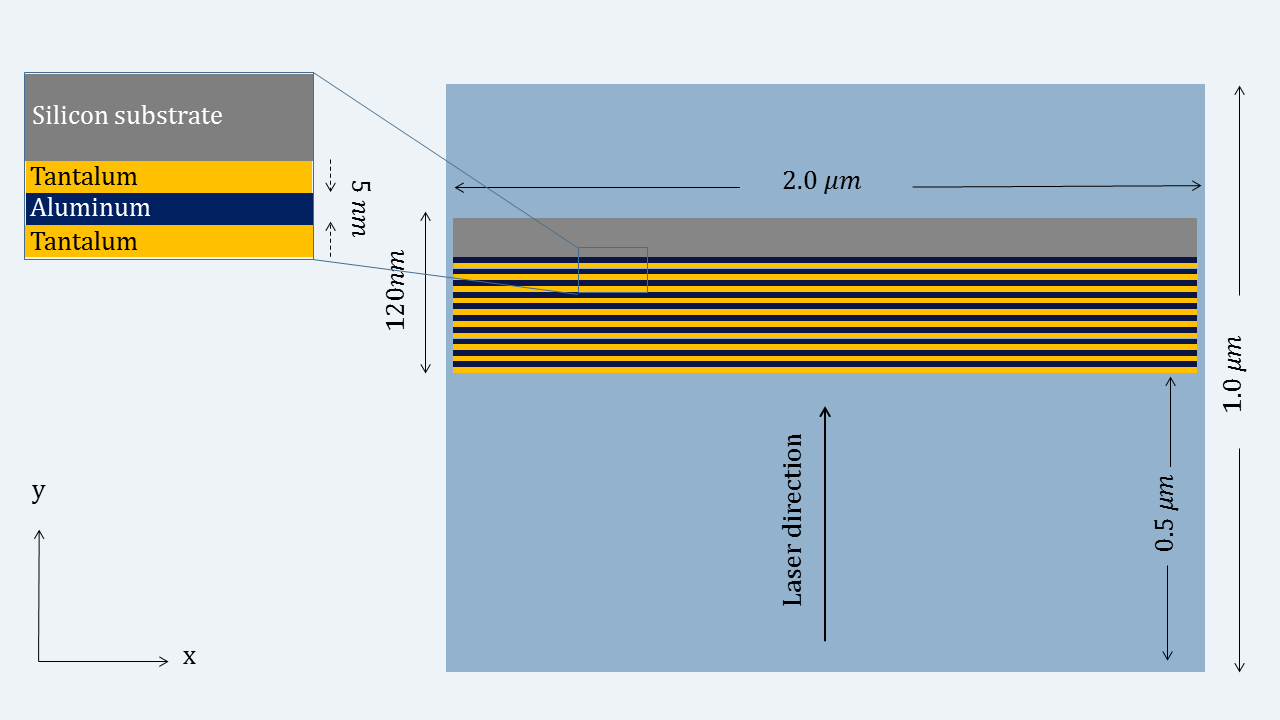
\includegraphics[width=0.8\linewidth]{P_2.png}
\caption{A schematic of PIC simulation setup}
\end{figure}

\subsection{X-ray diffraction}

\section{Results and discussion}
The figure (figure) is a closeup view the free (first row), bound (second row),
and total electron density (third row) 2D maps at 0, 75, 226, and 410 fs of the
PIC simulation. The maximum intensity of the lase pulse reaches the target at
the time 0 and it goes of the simulation box around 75 fs. One can easily see
the ionization process and generation of free electrons, reduction of bound
electrons, and the evolution of total electron density when the laser pulse
irradiates the target and even after that. Due to skin depth of Ta and Al the
laser pulse is not able to penetrate more than a few nanometer into the target
and will be partially reflected when it reaches the critical density, but due to
the laser ponderomotive force electrons at the front of target will be pushed
into the deeper layers. Regarding the high density of target, which is hundreds
of the critical density, and the intensity of laser the term of $\vec{J} \times
\vec{B}$ acceleration is negligible compare the dc-ponderomotive [reference].
However, due to penetration of laser into the skin depth, the magnetic part of
Lorentz force is able to drag some electrons and pull them out into the vacuum
causing the field is maintained zero inside the target [reference]. The most of
the dragged electrons will be pushed back into the target by inversing the laser
field during a cycle causing an oscillation perpendicular to the surface of the
target.

By following up the total electron density evolution in figure (figure), one can
easily see that the surface of the layers get more roughed and those roughness
become lager by the time. It also can be seen in figure (diffraction images),
which displays three diffraction pattern as a function of $Q$ in x and y
direction in ln-scale corresponding to -51.8, 160.3, and 341.9 fs. The
diffraction images show the specular signal as a high intensive streak and also
the diffuse scattering signal as a ring around the center by which we are able
to interpret the scale of the roughness. That means larger ring for diffuse
scattering signal corresponds to the smaller scale roughness and vice versa. By
this definition, we can relate the large ring at -51.8 fs to the angstrom scale
roughness which are mainly due to random distribution of particles inside the
angstrom scale simulation cells. By the time the ring gets smaller and for
larger $Q$-values there is only a weak scattering signal that means the scale of
the roughness gets lager due to the irradiation. This dynamic can also be seen
in figure (radial intensity figure a) shows a more detailed distribution of the
radial intensity of scattered X-ray as a function of $Q$ for different time from
-70 fs (red) to 395.9 fs (blue). Figure (radial intensity figure a) depicts the
maximum of the scattered intensity as a function of time displaying a reduction
of intensity until its minimum value at 124.6 fs that correspond to the three
quarter of optical laser pulse.

\begin{figure}[h]
\centering
\includegraphics[width=1.0\linewidth]{paper_plot.png}
\caption{2D electron density maps}
\end{figure}

The figure (figure) shows the averaged total electron density along the
transverse direction in which 0 fs shows the moment that peak of the laser pulse
reaches the surface of the target and 75.4 fs is right after the laser pulse. It
can obviously be seen that due to the radiation pressure during the laser pulse,
almost there is no expansion on the surface of the target. Besides that, the ML
target maintains its structure without significant change. After the laser pulse
at 75.4 fs see a few nanometer expansion of the electrons but latter due to the
hydrodynamic expansion, the surface expands rapidly up to 20 $nm$  until 226 fs,
and then with a lower speed up to 40 $nm$ until 452 fs. At the same time, the ML
structure is deformed by the distribution of the free electrons throughout the
target. This dynamic of electron density can also be seen in figure (contrast
figure) that shows the scattered X-ray intensity fluctuations by speckle
contrast $\beta$. As we mentioned earlier, the higher value of $\beta$
corresponds slower dynamics and it happens at the maximum intensity of the laser
pulse at 0 fs. Then, $\beta$ curve drops down rapidly that corresponds to
smaller intensity fluctuations and faster dynamics until 226 fs, from then it
the dynamics get faster with a slower speed. It is also shown in figure (Q as
time figure) that displays the variation of the Q-value as a function of time
for the maximum scattered X-ray intensity. Similar to the figure (contrast
figure), at 75.4 fs, right after the optical laser pulse, the Q-value drops down
to the 0.5 $nm^{-1}$ which means the scale of the roughness get larger during
this time. One can interpret the speed of the expansion from the slope of this
graph. For instance, from 75.4 to 200 fs, Q changes by 2 $nm^{-1}$ that
corresponds $\approx 1.5$ $nm$ in real space. Thus, the speed of the plasma
expansion during this time is about $10^{4}$ $m/s$.

\begin{figure}[h]
\centering
\includegraphics[width=0.8\linewidth]{Paper_plot_1D.png}
\caption{1D total electron density maps}
\end{figure}

To have a better image of these dynamics we considered some $Q$-rings with the
width of $\Delta Q \approx 0.08$ $nm^{-1}$ and different radius from 0.54 to
7.60 $nm^{-1}$ which are centered at the center of diffraction pattern ring as
it has been shown in figure (figure 5a of Lisa). The radius difference between
the rings is $\Delta Q_r \approx 0.08$ $nm^{-1}$. Figure (5b from Lisa) shows
the variation of the contrast $\beta$ for the smaller $Q$-rings up to radius
3.06 $nm^{-1}$ and figure (5c from Lisa) shows larger $Q$-rings. For the smaller
$Q$-rings which correspond to lagers scale roughness we see just a small
variation of contrast $\beta$. For instance, for 0.54 and 1.04 $nm^{-1}$,
corresponds to (length scale! ask Lisa) $nm$ in real space, one can just see
some fluctuations for $\beta$ by the time that means in large scale we are not
significant dynamics. But as we go to the larger $Q$-ring values there is an
obvious reduction of $\beta$ and faster dynamics for smaller scale roughness.

\section{Conclusion}

a short conclusion.

\section{Acknowledgment}
CFG acknowledges support from the European Cluster of Advanced Laser Light
Sources (EUCALL) project which has received funding from the European Union’s
Horizon 2020 research and innovation programme under grant agreement No 654220.

%\begin{equation}
%\label{eq:emc}
%e = mc^2
%\end{equation}

%\begin{figure}[h]
%\centering
\includegraphics[width=0.4\linewidth]{placeholder}
%\caption{Figure caption}
%\end{figure}

%\begin{table}[h]
%\centering
%\begin{tabular}{l l l}
%\hline
%\textbf{Treatments} & \textbf{Response 1} & \textbf{Response 2}\\
%\hline
%Treatment 1 & 0.0003262 & 0.562 \\
%Treatment 2 & 0.0015681 & 0.910 \\
%Treatment 3 & 0.0009271 & 0.296 \\
%\hline
%\end{tabular}
%\caption{Table caption}
%\end{table}
%% References
%%
%% Following citation commands can be used in the body text:
%% Usage of \cite is as follows:
%%   \cite{key}          ==>>  [#]
%%   \cite[chap. 2]{key} ==>>  [#, chap. 2]
%%   \citet{key}         ==>>  Author [#]

%% References with bibTeX database:
\bibliographystyle{model1-num-names}
\bibliography{references.bib, library.bib}


\end{document}

%%
%% End of file `elsarticle-template-1-num.tex'.
